% Section content template for individual Educative lessons
% This file contains the actual content for a specific section
% Generated from Educative API section content

% Section: Sequence Diagram for the Movie Ticket Booking System
% Section ID: 4835239549730816
% Section Slug: sequence-diagram-for-the-movie-ticket-booking-system
% Generated: 2025-12-12T14:19:45.423643

A sequence diagram is a great way to understand the interactions between different entities and objects in the system. There can be different sequence diagrams that we can create for our movie ticket booking system. In this lesson, we will create sequence diagrams for the following three interactions:

\begin{itemize}
\item
\protect\phantomsection\label{ZJUJawTcd_XPpaVIJFw5m}
\textbf{Create a booking:} The customer creates a booking for a show.
\item
\protect\phantomsection\label{KYicwvAyYS6LiRaFLgTsL}
\textbf{Payment for the booking:} The customer pays for the booking.
\item
\protect\phantomsection\label{rUTBXBMa0ok7dBgWBQ1wo}
\textbf{Sequence challenge:} The customer cancels their booking.
\end{itemize}

\subsection{Create a booking}\label{LbzN_f8ok7Qt_oyGTJ6Kz}
\\
The sequence diagram for creating a booking should have the following actors and objects that will interact with each other:

\begin{itemize}
\item
\protect\phantomsection\label{pnHplKAxUHicDBSf2Gbh4}
\textbf{Actor:} \texttt{Customer}
\item
\protect\phantomsection\label{p0WawNydj98mGeGkkMamK}
\textbf{Objects:} \texttt{Catalog}, \texttt{ShowTime}, and \texttt{Booking}
\end{itemize}
\\
Here are the steps of the interaction to create a booking:

\begin{enumerate}
\item
\protect\phantomsection\label{PlS5odQqNl9Ces87YXywq}
The customer searches for a movie from the catalog.
\item
\protect\phantomsection\label{vw8CdaZMTPvv_3wFgNB7f}
The catalog returns the required movie(s).
\item
\protect\phantomsection\label{X8la3TZQ2tMyWA_zPRWCq}
The customer requests showtimes for the selected movie from the catalog.
\item
\protect\phantomsection\label{G9UVc_Mhs2vcOz9Xv4cnX}
The available showtimes for the movie are returned.
\item
\protect\phantomsection\label{t_HQpzGuYS3xpcJ7WExXf}
The customer requests available seats for the selected showtime.
\item
\protect\phantomsection\label{qMhvonkBTcBeOFyVF0zki}
If seats are available:

\begin{enumerate}
\item
The customer receives a list of available seats.
\item
The customer selects their desired seats and requests to create a booking.
\item
The booking is created for the customer, selected seats, and showtime. The booking status is set to ``PENDING.''
\item
The customer is notified that the booking is created and that payment is required.
\end{enumerate}
\item
\protect\phantomsection\label{luI3gNQnHVnHJSktC03uo}
Else if no seats are available:

\begin{enumerate}
\item
The customer is informed that no seats are available.
\end{enumerate}
\end{enumerate}
\\
Based on the order above, the sequence diagram for creating a booking in the movie ticket booking system is given below.

\begin{figure}[htbp]
 \centering
 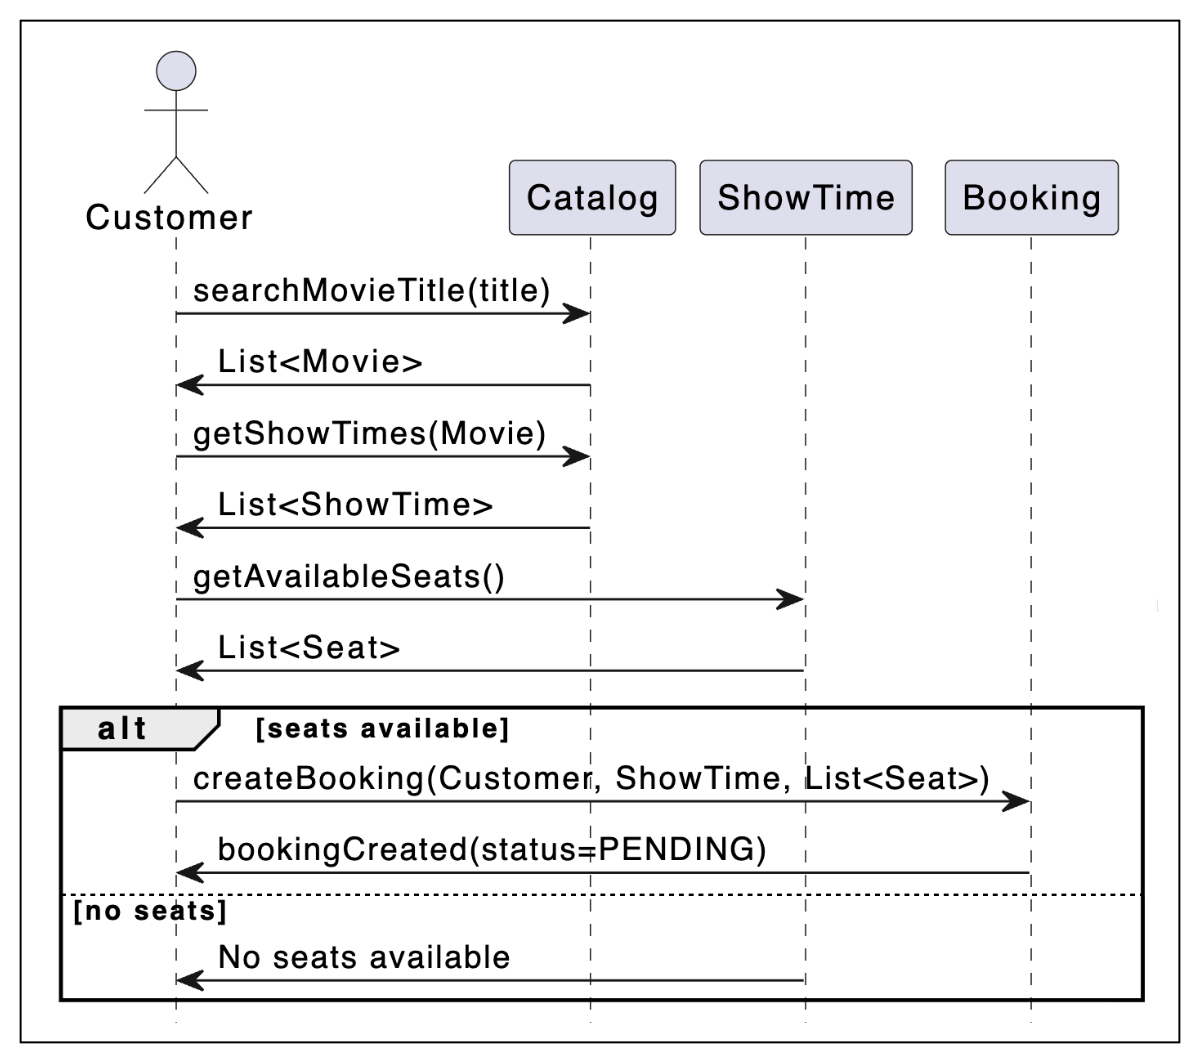
\includegraphics[width=0.5\textwidth]{Images/chapter_14/section_4835239549730816/6462309453922304.png}
 \caption{The sequence diagram to create a booking }
\end{figure}

\subsection{Payment of a booking}\label{Xe5USwZbVn0XpSoRnrBIg}
\\
The sequence diagram for payment of a booking should have the following actors and objects that will interact with each other:

\begin{itemize}
\item
\protect\phantomsection\label{vriIgYn_EV5zmPg01ogg8}
\textbf{Actor:} \texttt{Customer}
\item
\protect\phantomsection\label{W5HowvyRrOLlXpRzioRGX}
\textbf{Objects:} \texttt{Booking}, \texttt{Payment}, and \texttt{Notification}
\end{itemize}
\\
Here are the steps in the payment of a booking interaction:

\begin{enumerate}
\item
\protect\phantomsection\label{FimxLDplGkI4WiQpVEh7C}
The customer initiates a payment for the booking fee through the booking system.
\item
\protect\phantomsection\label{XREtR88wDuM-x9rPxYxsq}
The booking system creates a payment object and processes the payment.
\item
\protect\phantomsection\label{_un0Spk-a07C8xazjG9LY}
If the payment is confirmed:

\begin{enumerate}
\item
The payment informs the system about the successful payment.
\item
The booking status is updated to ``CONFIRMED.''
\item
The system sends a notification to the customer containing the booking confirmation.
\end{enumerate}
\item
\protect\phantomsection\label{vhJhnIcdQuK7iX-PkyWN-}
Else if the payment is declined:

\begin{enumerate}
\item
The payment informs the system about the declined payment.
\item
The booking status is updated to ``DECLINED.''
\item
The system sends a notification to the customer that the booking has been declined.
\end{enumerate}
\end{enumerate}
\\
Based on the order above, the sequence diagram for payment of a booking in the movie ticket booking system is given below.

\begin{figure}[htbp]
 \centering
 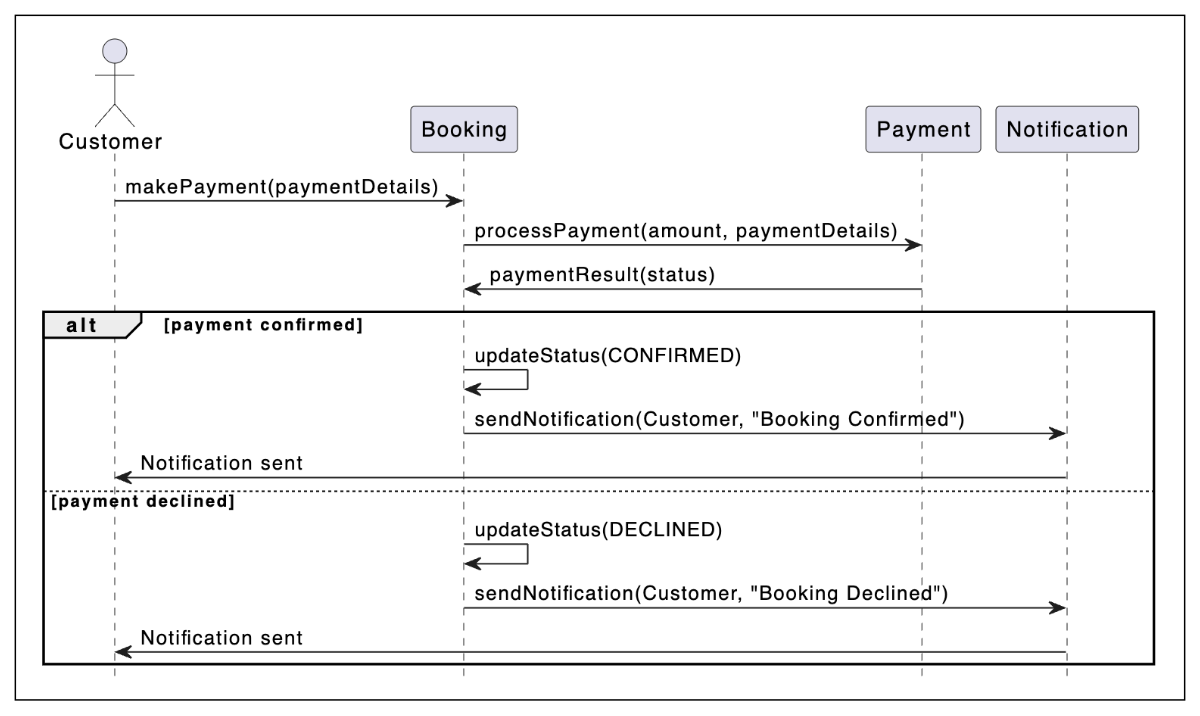
\includegraphics[width=0.5\textwidth]{Images/chapter_14/section_4835239549730816/4945012285374464.png}
 \caption{The sequence diagram for the payment of a booking interaction}
\end{figure}

\subsection{Sequence challenge: Cancel booking}\label{3VLpXbIWQX-WuMx2zTsmy}
\\
You will complete a sequence diagram for a booking canceled by the customer. A skeleton of the cancel sequence diagram is given below:

\begin{figure}[htbp]
 \centering
 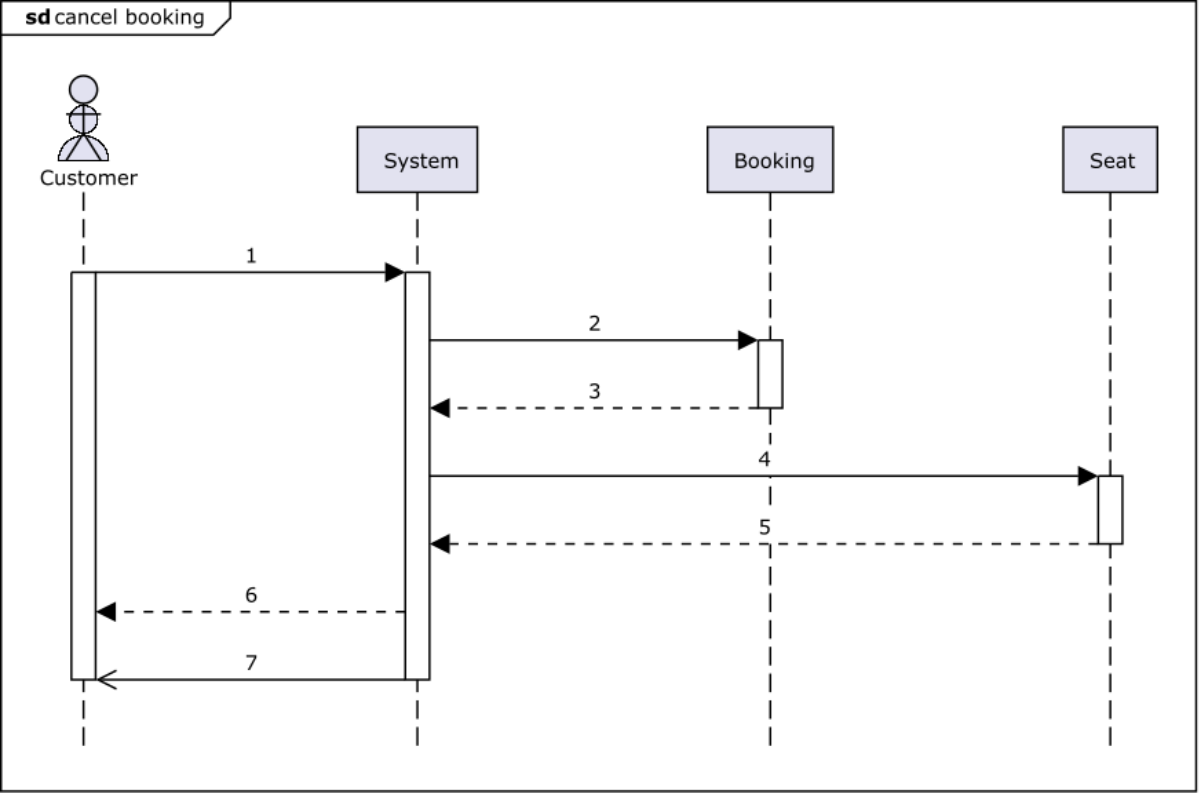
\includegraphics[width=0.5\textwidth]{Images/chapter_14/section_4835239549730816/5698570382737408.png}
 \caption{The sequence diagram for canceling the booking}
\end{figure}

Notice that the arrows in the diagram above are numbered from 1 to 7. The message boxes shown below are the messages to be exchanged between the actor(s) and object(s). Can you rearrange the messages below in the correct sequence in order they should appear in the skeleton of the sequence diagram given above?
\begin{quote}
\textbf{Note:} If you're stuck, click the ``Show Solution'' button.
\end{quote}

Alternatively, you can also click the ``Show complete diagram'' button below to see the complete sequence diagram for the cancel booking interaction.

Next, let's examine the activity diagrams for the movie ticket booking system to understand its control flow.

% End of section content